\documentclass[12pt]{article} 
\usepackage{fancyhdr}
\usepackage[margin=1.9cm]{geometry}
\usepackage{parskip}
\usepackage{amsmath}
\usepackage{amssymb}
\usepackage{enumerate}
\usepackage{graphicx}
\graphicspath{ {} }
\usepackage{times} %Times New Roman

\begin{document}
\pagestyle{fancy}
\rhead{AQM Problem Set 2 - Ismael Martinez} 
\renewcommand{\headrulewidth}{0pt}

\section{Maximum Likehood  for Linear Regression}
We consider the simple linear regression model $\,Y = \beta_0 + \beta_1X + \epsilon\,$ with $n$ observation points $(x_1, y_1), \dots ,(x_n, y_n)\,$ and $\epsilon \sim \mathcal{N}(0,\sigma^2)$. 
We estimate $\beta_0$, $\beta_1$ and $\sigma^2$ by $b_0$,$b_1$, and $s^2$ respectively which we have chosen. For a certain response $y_i$, we want to find the probability of observing this response 
given our chouse in parameters. We get 
\begin{equation*}
	P(y_i\, | \, x_i ; b_0, b_1, s^2) = \frac{1}{\sqrt{2\pi s^2}}e^{-\frac{(y_i - (b_0 + b_1x_1))^2}{2s^2}} .
\end{equation*}
What we are calculating here is the probability of the error $\epsilon$ covering the difference between $y_i$ and $ b_0 + b_1x_i$. Similarly, for the probability of observing the entire dataset, we obtain 
\begin{equation*}
	\prod\limits_{i=1}^n P(y_i\, | \, x_i ; b_0, b_1, s^2) .
\end{equation*}
We can take the log to get 
\begin{equation*}
\mathcal{L}(b_0,b_1,s^2) = \log \prod\limits_{i=1}^n P(y_i\, | \, x_i ; b_0, b_1, s^2) = \sum\limits_{i=1}^n \log P(y_i\, | \, x_i ; b_0, b_1, s^2).
\end{equation*}
Finally, we can maximize the above equation to get the estimators.
\begin{align*}
\hat{\beta_1} &= \frac{\sum\limits_{i=1}^n (x_i - \bar{x})(y_i - \bar{y})}{\sum\limits_{i=1}^n (x_i - \bar{x})(x_i - \bar{x})} \\
\hat{\beta_0} &= \bar{y} - \hat{\beta_1}\bar{x} \\
\hat{\sigma^2} &= \frac{1}{n} \sum \limits_{i=1}^n (y_i - (\hat{\beta_0} + \hat{\beta^1}x_i))^2
\end{align*}

\section{Optimizing the Likelihood Function}
The scripts are provided in \texttt{gradientDescent.R} and \texttt{likelihoodFunction.R}.

\section{Model Validation Methods}
\begin{enumerate}
\item
	Through the script written in \texttt{P2\_3.R}, we find the table of predictions.
\begin{center}
	\begin{tabular}{|c|c|c|}
	\hline
	& \multicolumn{2}{|c|}{True} \\
	\hline 
	Pred & 0 & 1 \\
	\hline
	0 & 434 & 11 \\
	\hline 
	1 & 10 & 228\\
	\hline
	\end{tabular}
	\end{center}
	From this table, we get a total misclassification percentage of approximately $3.07\%$.	

\item
	Through the script written in \texttt{P2\_3\_2.R}, we find the table of predictions. For the training/testing split, I used a 70/30 split.
\begin{center}
	\begin{tabular}{|c|c|c|}
	\hline
	& \multicolumn{2}{|c|}{True} \\
	\hline 
	Pred & 0 & 1 \\
	\hline
	0 & 133 & 5 \\
	\hline 
	1 & 2 & 66\\
	\hline
	\end{tabular}
	\end{center}
	From this table, we get a total misclassification percentage of approximately $3.40\%$.	

\item
	From \texttt{P2\_3\_3.R}, we calculate 10-Fold cross-validation and get a misclassification percentage of $3.35\%$.

\item
We use the script in \texttt{P2\_3\_4.R} to see the error image in Figure 1. The training error appears to be monotonically increasing, so in this case it is best to use a low value for $K$ around $2,3$ or $4$.
\begin{figure}
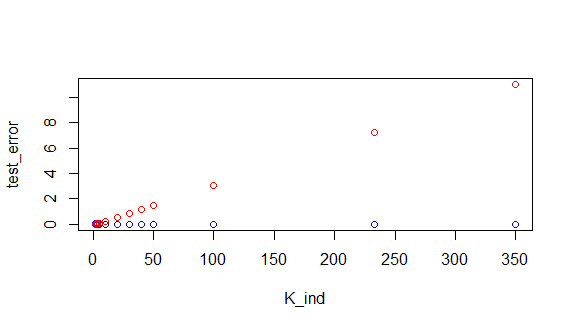
\includegraphics{Rplot}
\caption{Red: Train Error, Blue: Test Error}
\end{figure}

\end{enumerate}

\section{Cross-Validation Intuition}
In this case, I would choose the second method. The reason is that LOOCV has high variance, and if the dataset has 10,000 predictor variables, it is likely to be large in row size as well making LOOCV computationally expensive. In the second method, we drop the variables with the lowest variance, meaning 
the variables are relatively unchanging and have little effect on the response variable. Although only variables with relatively higher variance remain, 10-fold cross validation does not inherintly have high variance, so this variance is kept under control.  


\end{document}